\documentclass[../../../../main.tex]{subfiles}
\begin{document}

\begin{flushright}
\footnotesize\textit{【自動文字起こし・要確認】}
\end{flushright}

\noindent
\textbf{[解]} $S = \sin t, C = \cos t$ とする。\\
$f(t) = 2C + \cos 2t$, $g(t) = \sin 2t$ とおく。

\bigskip
\noindent
(1) $f'(t) = -2S - 2\sin 2t$, $g'(t) = 2\cos 2t$ だから、$\vec{v} = \begin{pmatrix} f'(t) \\ g'(t) \end{pmatrix}$ とすると、
\begin{align*}
|\vec{v}|^2 &= 4(S + \sin 2t)^2 + 4\cos^2 2t \\
&= 4S^2 + 8S \sin 2t + 4 \\
&= 4S^2(1 + 4C) + 4 \\
&= 4[(1-C^2)(1+4C) + 1] \equiv h(C)
\end{align*}
とおく。\\
$h'(C) = -2(6C^2 + C - 2) = -2(3C+2)(2C-1)$ から、下表を得る。

\begin{center}
\begin{tabular}{c|ccccccc}
$C$ & $-1$ & $\dots$ & $-\frac{2}{3}$ & $\dots$ & $\frac{1}{2}$ & $\dots$ & $1$ \\ \hline
$h'$ & & $-$ & $0$ & $+$ & $0$ & $-$ & \\ \hline
$h$ & $4$ & $\searrow$ & $\frac{8}{27}$ & $\nearrow$ & $13$ & $\searrow$ & $4$
\end{tabular}
\end{center}

したがって $|\vec{v}| \ge 0$ より、$\max |\vec{v}| = \sqrt{13}$, $\min |\vec{v}| = \sqrt{\frac{8}{27}}$ \quad \text{\#\#}

\bigskip
\noindent
(2) $f'(t) = -2S(1+2C)$, $g'(t) = 2\cos 2t$ から下表を得る。($f(\pi+t) = f(\pi-t), g(\pi+t) = -g(\pi-t)$)

\begin{center}
\begin{tabular}{c|ccccccccc}
$t$ & $0$ & $\dots$ & $\pi/4$ & $\dots$ & $\frac{2}{3}\pi$ & $\dots$ & $\frac{3}{4}\pi$ & $\dots$ & $\pi$ \\ \hline
$f'$ & $0$ & $-$ & $-$ & $-$ & $0$ & $+$ & $+$ & $+$ & $0$ \\ \hline
$g'$ & $+$ & $+$ & $0$ & $-$ & $-$ & $-$ & $0$ & $+$ & $+$ \\ \hline
$(x,y)$ & $(3,0)$ & $\searrow$ & $(\sqrt{2},1)$ & $\swarrow$ & & $\nwarrow$ & & $\nearrow$ & $(-1,0)$
\end{tabular}
\end{center}

したがって、グラフの概形は下図のようになる。

\begin{center}
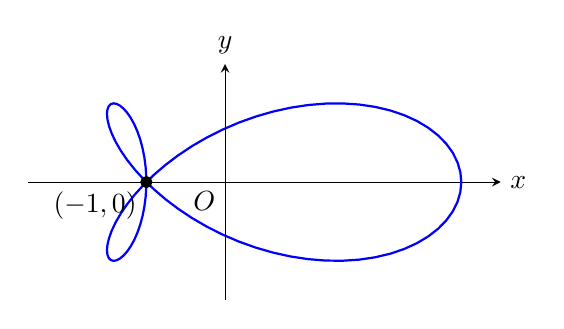
\begin{tikzpicture}[scale=1.0, >=stealth]
  \draw[->] (-2.5,0) -- (3.5,0) node[right] {$x$};
  \draw[->] (0,-1.5) -- (0,1.5) node[above] {$y$};
  \node[below left] at (0,0) {$O$};

  \draw[thick, blue, domain=0:2*pi, samples=100] plot ({2*cos(\x r) + cos(2*\x r)}, {sin(2*\x r)});
  \filldraw (-1,0) circle (2pt) node[below left] {$(-1,0)$};
\end{tikzpicture}
\end{center}

ここで、$(f(t), g(t))$ ($0 \le t < 2\pi$) の表す曲線の交点が $(-1,0)$ のみであることを示す。$f(t), g(t)$ の増減及び対称性から、$0 < t < \pi$ の時に共有点がないことを示せば良い。背理法で示す。$t_1, t_2$ に対応する点で交わっているとすると ($t_1 < t_2$)
\[
\begin{cases}
2\cos t_1 + \cos 2t_1 = 2\cos t_2 + \cos 2t_2 & \dots \text{①} \\
\sin 2t_1 = \sin 2t_2 & \dots \text{②}
\end{cases}
\]
$\frac{\pi}{2} < t_1 < t_2 < \pi$ 及び ② から、$t_2 = \frac{3}{2}\pi - t_1$ である。この時 ① から
\begin{align*}
& 2\cos t_2 + \cos 2t_2 = -2\cos \left(\frac{\pi}{2} - t_1\right) - \cos 2t_1 = 2\cos t_1 + \cos 2t_1 \\
\implies & \sin t_1 + \cos t_1 + 2\cos 2t_1 = 0
\end{align*}
だから $\sin^2 t_1 + \cos^2 t_1 = 1$ に代入して、以下 $P = \cos t_1$ とすると
\[
P(P+1)(5P^2 - P - 2) = 0 \quad \dots \text{③}
\]
一方、$\frac{\pi}{2} < t_1 < t_2 < \pi$ だったから $t_2 = \frac{3}{2}\pi - t_1$ から
\[
\frac{\pi}{2} < t_1 < \frac{3}{4}\pi
\]
だから $-\frac{\sqrt{2}}{2} < P < 0$ となる。③ を同時にみたす $P$ はなく矛盾。

\bigskip
\noindent
以上から、交点はただ1つ存在し、同時刻 $t = \frac{\pi}{2}, \pi, \frac{3}{2}\pi$ での速度ベクトルは各々
\[
\begin{pmatrix} -2 \\ -2 \end{pmatrix}, \quad \begin{pmatrix} 0 \\ 2 \end{pmatrix}, \quad \begin{pmatrix} 2 \\ -2 \end{pmatrix}
\]
だから図示して下図。

\begin{center}
\begin{tikzpicture}[scale=1.0, >=stealth]
  \draw[->] (-3,0) -- (2,0) node[right] {$x$};
  \draw[->] (0,-3) -- (0,3) node[above] {$y$};
  \filldraw (-1,0) circle (2pt) node[above left] {$(-1,0)$};

  \draw[->, ultra thick, red] (-1,0) -- (-1,2) node[above] {$(0,2)$};
  \draw[->, ultra thick, red] (-1,0) -- (-3,-2) node[below left] {$(-2,-2)$};
  \draw[->, ultra thick, red] (-1,0) -- (1,-2) node[below right] {$(2,-2)$};
\end{tikzpicture}
\end{center}

\bigskip
\noindent
\textbf{[解2] (交点の唯一性)}\\
②から $t_1, t_2 = \frac{3}{4}\pi \pm \alpha$ ($0 < \alpha < \frac{3}{4}\pi$) とおける。$f(t) = 2C^2 + 2C - 1$ だから
\[
f\left(\frac{3}{4}\pi \pm \alpha\right) = -\sqrt{2}\cos\alpha \pm (1-\sqrt{2})\sin\alpha - 1
\]
これらが一致することはないので不適。 \quad \text{\#\#}

\end{document}
